\documentclass{project}
\usepackage[pdfauthor={C. P. Marriott},pdftitle={Software Engineering Group Project, Project Plan},pdftex]{hyperref}
\usepackage[pdftex]{graphicx}
\usepackage{pdfpages}
\hypersetup{colorlinks=false,pdfborder={0 0 0}}
\begin{document}
\title{Software Development Life cycle}
\subtitle{Testing Specification}
\author{Tom Reed, Matt Whitmore, Dave Clark, Silhab Csoma, Mike Steel, Chris 'Tux' Lloyd, Aleksandra Badyda, Samuel Jackson, Chris Marriott}
\shorttitle{Testing Specification}
\version{1.4}
\status{Finalised}
\date{2013-1-28}
\configref{SE.17.DS.01}
\maketitle
\tableofcontents
\newpage
\section{Introduction}
\subsection{Purpose of this Document}
By producing this document we shall explain any and all tests to be carried out on our project prior to it being considered finished, all tests shall cover necessary functions of the project and allow us to discover any errors or defects before it is put into use. 
\subsection{Scope}
This document specifies the tests that will be run to discover various bugs and put general strain on
the system. It will in detail outline the tests that will be run and the required outcome as well as what
will constitute a failed test. This document will also outline what will be done with the test data and
how it will be reported.
\subsection{Objectives}
The objective of this document is to outline the tests that will be run on the system, how they will be
structured and how they will be documented and reported.

\section{Test Plan}
\subsection{Test Overview}
An HTTP servlet is used to access the data contained within the backend of the server as if it was almost a web page.  We will pass parameters between it and get a response. We will be working on the principle that one main servlet will perform different actions, passing through an actions variable and any data required to be processed. There are two methods of accessing this; using �get� and �post� requests.  The get request will pass the parameters through the URL, the post request through a hidden layer, based on the users input. JavaScript will collate the necessary data, and attach the appropriate action command before sending to the server.
All coders will be responsible for testing their code, code will be tested using a set of JUnit tests. As the code has not been written yet it is impossible to stipulate at this time what the tests will need to be. HTML and CSS will be tested using the W3C validators as well as tested in various browsers that support HTML5. For the system testing, we need to test it through the client side as there is no real
way access the server side of the system without using JUnit testing which has already been
stipulated. So the only way to approach it is to test if the server side does as we expect from the
client side.
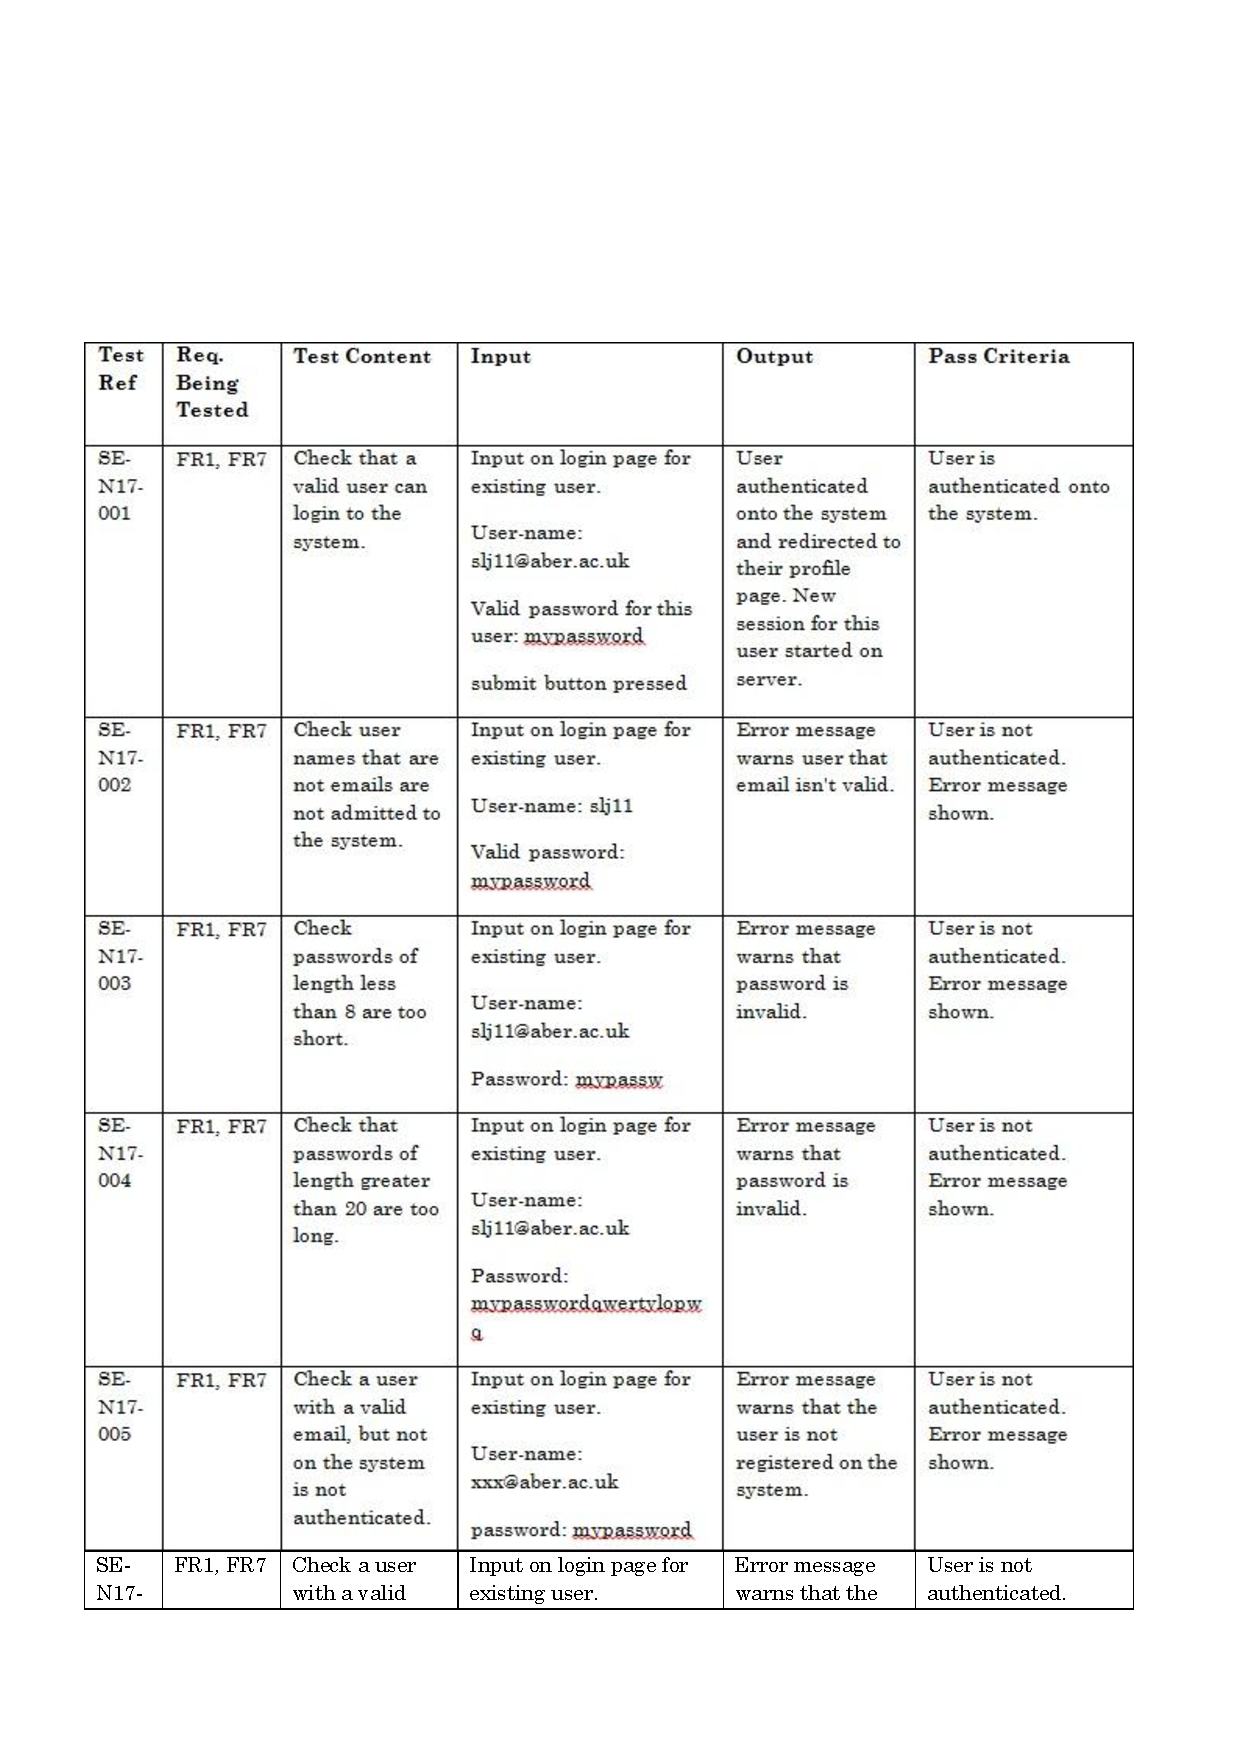
\includepdf[pages=1,pagecommand=\subsection{Test Specification}]{Test_spec.pdf}
\includepdf[pages=2-,pagecommand={}]{Test_spec.pdf}

\subsection{Test Result Reporting}
Test results will be recorded in a test log form (included on the next page). These documents will be
stored in the groups Github repository under the folder �Test Data�, there will be two sub folders with
in this directory called �Module Tests� and �System Tests�. The corresponding test documents will be
stored into those two directories.

\subsection{Configurations}
Using Github we can branch off from the master copy of the project for testing and working on, doing
this will insure that everyone is using the same version of the project. This is to make sure that
everyone runs their tests on the same copy of the project insuring consistency. Branching off from the
master copy will also allow for version roll back. Meaning that if a mistake is made and the system no
longer works. We can return to a stable version when we know it works.
\newpage

\section{Test Log Form}
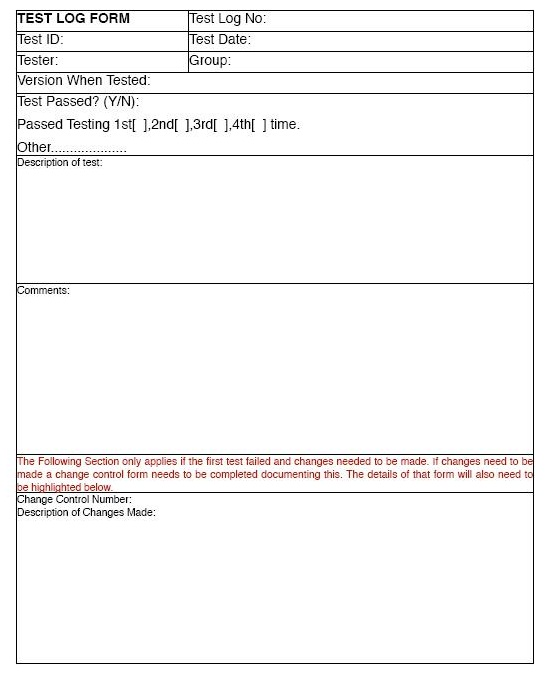
\includegraphics{project2_testlog.jpg}

\addcontentsline{toc}{section}{DOCUMENT HISTORY}
\section*{DOCUMENT HISTORY}
\begin{tabular}{|l | l | l | l | l |}
\hline
Version & CCF No. & Date & Changes made to Document & Changed by \\
\hline
1.0 & N/A & 2012-10-31 & Initial creation & CPM4 \\
\hline
1.1 & N/A & 2012-11-2 & Added information from Mike & CPM4 \\
\hline
1.2 & N/A & 2012-12-5 & Updated config ref and added other documents & CPM4 \\
\hline
1.3 & N/A & 2012-12-6 & Added missing data and fixed few mistakes & CPM4 \\
\hline
1.4 & N/A & 2013-1-28 & Made advised changes as per blackboard & MIS28 \\
\hline
\end{tabular}
\label{thelastpage}
\end{document}

